% Created 2019-10-16 Wed 04:53
% Intended LaTeX compiler: pdflatex
\documentclass[nobib]{tufte-handout}


\usepackage{minted}
\usepackage{ifluatex, ifxetex}
%Next block avoids bug, from http://tex.stackexchange.com/a/200725/1913
\ifx\ifxetex\ifluatex\else
\newcommand{\textls}[2][5]{%
\begingroup\addfontfeatures{LetterSpace=#1}#2\endgroup
}
\renewcommand{\allcapsspacing}[1]{\textls[15]{#1}}
\renewcommand{\smallcapsspacing}[1]{\textls[10]{#1}}
\renewcommand{\allcaps}[1]{\textls[15]{\MakeTextUppercase{#1}}}
\renewcommand{\smallcaps}[1]{\smallcapsspacing{\scshape\MakeTextLowercase{#1}}}
\renewcommand{\textsc}[1]{\smallcapsspacing{\textsmallcaps{#1}}}
% shove everything else in here so we don't mess with emacs latexpreview, which doesn't use lualatex
\usepackage{fontspec}
\setmainfont{ETBookOT}
\setmonofont[Scale=0.8]{Fantasque Sans Mono}
\renewcommand{\contentsname}{Contents}
\titleformat{\chapter}%
[display]% shape
{\relax\ifthenelse{\NOT\boolean{@tufte@symmetric}}{\begin{fullwidth}}{}}% format applied to label+text
{\huge\thechapter}% label
{0pt}% horizontal separation between label and title body
{\huge\rmfamily}% before the title body
[\ifthenelse{\NOT\boolean{@tufte@symmetric}}{\end{fullwidth}}{}]% after the title body
\titleformat{\section}%
[hang]% shape
{\normalfont\Large}% format applied to label+text
{\thesection}% label
{1em}% horizontal separation between label and title body
{}% before the title body
[]% after the title body
\titleformat{\subsection}%
[hang]% shape
{\normalfont\large\itshape}% format applied to label+text
{\thesubsection}% label
{1em}% horizontal separation between label and title body
{}% before the title body
[]% after the title body
\renewcommand{\maketitle}{%
\begingroup
\setlength{\parindent}{0pt}%
\setlength{\parskip}{4pt}%
\LARGE\scshape\plaintitle\par
\Large\itshape\plainauthor\par
\Large\itshape\thedate\par
\endgroup
%\thispagestyle{plain}% suppress the running head
%\tuftebreak
%\@afterindentfalse\@afterheading% suppress indentation of the next paragraph
}
\usepackage{graphicx}
\fi
\newcommand{\xv}[0]{\mathbf{x}}
\newcommand{\yv}[0]{\mathbf{y}}
\newcommand{\zv}[0]{\mathbf{z}}
\newcommand{\fv}[0]{\mathbf{f}}
\newcommand{\J}[0]{\mathbf{J}}
\newcommand{\gv}[0]{\mathbf{g}}
\newcommand{\hv}[0]{\mathbf{h}}
\newcommand{\hxo}[0]{\mathbf{h}_0}
\usepackage{mathtools}
\DeclarePairedDelimiter\abs{\lvert}{\rvert}%
\DeclarePairedDelimiter\norm{\lVert}{\rVert}%
% Swap the definition of \abs* and \norm*, so that \abs
% and \norm resizes the size of the brackets, and the
% starred version does not.
\makeatletter
\let\oldabs\abs
\def\abs{\@ifstar{\oldabs}{\oldabs*}}
%
\let\oldnorm\norm
\def\norm{\@ifstar{\oldnorm}{\oldnorm*}}
\makeatother
\newcommand*{\approxident}{%
\mathrel{\vcenter{\offinterlineskip
\hbox{$\sim$}\vskip-.35ex\hbox{$\sim$}\vskip}}}
\author{James Gilles}
\date{11 October 2019}
\title{18.337 homework 1}
\hypersetup{
 pdfauthor={James Gilles},
 pdftitle={18.337 homework 1},
 pdfkeywords={},
 pdfsubject={},
 pdfcreator={Emacs 26.3 (Org mode 9.2.6)}, 
 pdflang={English}}
\begin{document}

\maketitle
\tableofcontents


\section{Problem 1}
\label{sec:orgc11fc44}
\subsection{Part 1}
\label{sec:orgca8ca0b}
We want to show that if \(\xv^*\) is a fixed point of newton's method, then \(\gv(\xv^*) = \mathbf{0}\).
We have:

$$\xv^* = \xv^* - \left(\J_{\gv}(\xv^*)\right)^{-1} \gv(\xv^*)$$

Therefore:

$$\left(\J_{\gv}(\xv^*)\right)^{-1} \gv(\xv^*) = \mathbf{0}$$

\(\J_{\gv}(\xv^*)\) is invertible by definition, so its nullspace has only one element, \(\mathbf{0}\). So \(\gv(\xv^*) = \mathbf{0}\).

\marginnote[-1.5in]{Geometrically, we're drawing a line up to \(\gv(\xv^*)\), drawing a tangent line along \(\gv'(\xv^*)\), and moving to the x-intersect of that line. It's only possible for the x-intersect of that line to be \(\xv^*\) if \(\gv(\xv^*)\) is already \(\mathbf{0}\). This analogy also works in higher dimensions, although it's harder to visualize.}

\subsection{Part 2}
\label{sec:org4315634}

The quasi-newton approximation is of the form:

$$\xv_{n+1} = \xv_n - \left(\J_{\gv}(\xv_0)\right)^{-1} \gv(\xv_n) = \hxo(\xv_n)$$

where \(\hxo\) denotes the update step using the Jacobian from some particular point \(\xv_0\).

We want to determine a condition for which this sequence is stable, that is, for which it approaches a fixed point.
Let's assume that \(\gv \in C^2\) (and therefore that \(\hxo \in C^2\)), that \(\J_{\hxo}\) is nonsingular, and that a fixed point \(\xv^*\) of \(\hxo\) exists.

Let us also assume that, for all eigenvalues \(\lambda_{i}\) of the Jacobian \(\J_{\hxo}(\xv^*)\), \(\abs{\lambda_i} \leq 1\). Because \(\hxo\) is continuous,
this property holds for some connected neighborhood around \(\xv^*\).

Now, given some points \(\xv\) and \(\yv\) in the neighborhood, we have:

$$\norm{\hxo(\yv) - \hxo(\xv)}=\norm{\int_{\xv}^{\yv} \J_{\hxo}(\zv)\; d\zv}$$
$$\leq\int_{\xv}^{\yv} \norm{\J_{\hxo}(\zv) \; d\zv} < \int_{\xv}^{\yv} \norm{1 \; d\zv} = \norm{\xv - \yv}$$

\marginnote[-0.5in]{Note: The value of this line integral is unique, because each of the Jacobian's rows forms a conservative vector field.}

So we have:

$$\norm{\hxo(\yv) - \hxo(\xv)} < \norm{\xv - \yv}$$

That is, in the neighborhood of \(\xv^*\), \(\hxo\) is a contraction mapping. Therefore, by the Banach fixed point theorem, it must be stable around \(\xv^*\).

Now we can ask: concretely, what do the eigenvalues of \(\J_{\hxo}\) look like? We can compute:

$$\J_{\hxo}(\xv)
   = \left(\xv - \left(\J_{\gv}(\xv_0)\right)^{-1} \gv(\xv)\right)'
   = I - \left(\left(\J_{\gv}(\xv_0)\right)^{-1}\gv(\xv)\right)'
   $$

Diagonalize to rewrite this last term as:

$$I - P^{-1}DP$$

Now note:

$$I - P^{-1}DP = P^{-1}IP - P^{-1}DP = P^{-1}(I - D)P$$

So the eigenvalues of $$\J_{\hxo}(\xv)$$ are equal to 1 minus the eigenvalues of \(\left(\left(\J_{\gv}(\xv_0)\right)^{-1}\gv(\xv)\right)'\).

Therefore, for the sequence to converge, \(\left(\left(\J_{\gv}(\xv_0)\right)^{-1}\gv(\xv)\right)'\) should have eigenvalues in the range \((0,2)\),
and \(\xv_0\) should be near \(\xv^*\). If these properties hold, then the sequence will converge to \(\xv^*\).

\subsection{Part 3}
\label{sec:org3a5bc6b}
The proof is the same as before, but \(\alpha\) can be tuned to put the eigenvalues of \(\alpha\left(\left(\J_{\gv}(\xv_0)\right)^{-1}\gv(\xv)\right)'\) in
the range \((0, 2)\) as long as those eigenvalues are positive.

\subsection{Part 4.}
\label{sec:org76690ae}
\begin{enumerate}
\item Define \(\hv(\xv) = \xv^* - \gv(\xv^* - \xv)\). Then \(\hv(\mathbf{0}) = \mathbf{0}\).

\item Change \(\xv_0\) to \(\xv^*\); then you're approximating the fixed-point iteration. Basically, quasi-newton will converge worse if there are larger eigenvalues at \(\xv_0\).
\end{enumerate}

\newpage
\section{Problem 2}
\label{sec:org043a819}
\subsection{Part 1}
\label{sec:org4bcbce0}
\begin{minted}[frame=lines,linenos=true,mathescape,breaklines=true]{julia}
   using Plots, ForwardDiff, StaticArrays, Distributions, Test
   pyplot()

   is_close(x,y) = abs(x - y) < .0000001

   function newton_quantile(cdf, y, x0; maxsteps=10000, pdf=x -> ForwardDiff.derivative(cdf, x))
       f = x -> cdf(x) - y
       x = x0
       for _ in 1:maxsteps
           px = x
           df = pdf(x)
           x = x - df \ f(x)
           if is_close(x, px)
               return x
           end
       end
       error("newton's method did not converge in step limit")
   end

   @test newton_quantile(x -> x, .2, .5) == .2
   @test newton_quantile(x -> x, .3, .5) == .3
   @test newton_quantile(x -> x, .9, .5) == .9
\end{minted}

\subsection{Part 2}
\label{sec:org1b6fadf}
\begin{minted}[frame=lines,linenos=true,mathescape,breaklines=true]{julia}
   function my_quantile(d, y; x0 = mean(d), maxsteps=10000)
       newton_quantile(x -> cdf(d, x), y, x0, maxsteps=maxsteps,
                       pdf=x -> pdf(d, x))
   end

   for d in [Gamma(5, 1), Normal(0, 1), Beta(2, 4)]
       for y in range(0.01, .99, length=100)
           @test is_close(my_quantile(d, y), quantile(d, y))
           @test is_close(my_quantile(d, y), quantile(d, y))
       end
   end
\end{minted}

\newpage
\section{Problem 3}
\label{sec:org9de8a01}
\subsection{Part 1}
\label{sec:org100afe3}
\begin{minted}[frame=lines,linenos=true,mathescape,breaklines=true]{julia}
   function calc_attractor!(out,r;warmup=400,x0=0.25)
       x = x0
       for _ in 1:warmup
           x = r * x * (1 - x)
       end
       for i in 1:length(out)
           out[i] = x
           x = r * x * (1 - x)
       end
   end
   out = zeros(150)
   calc_attractor!(out, 2.9)

   @test is_close(out[1], (2.9 - 1) / 2.9)
\end{minted}

\subsection{Part 2}
\label{sec:org51f9e11}
\begin{minted}[frame=lines,linenos=true,mathescape,breaklines=true]{julia}
   n = 1000
   rs = 2.9:0.001:4

   function calc_serial(n, rs; warmup=400)
       out = zeros(n, length(rs), 2)

       for (i, r) in enumerate(rs)
           out[:, i, 1] .= r
           slice = @view out[:, i, 2]
           calc_attractor!(slice, r, warmup=warmup)
       end
       out
   end

   function bifurcation_plot(out)
       xs = reshape(out[:, :, 1], :)
       ys = reshape(out[:, :, 2], :)

       plot(xs, ys, markershape=:rect, markerstrokewidth=0,
            markersize=0.8, markercolor=:black, markeralpha=0.01,
            line=false, legend=false, foreground_color_border=:transparent,
            foreground_color_axis=:transparent, format=:png, dpi=400,
            seriestype=:scatter, title="Bifurcations", fontfamily="ETBookOT")
   end

   savefig(bifurcation_plot(calc_serial(n, rs)), "bifurcation.png")
\end{minted}

\begin{figure*}
\centering
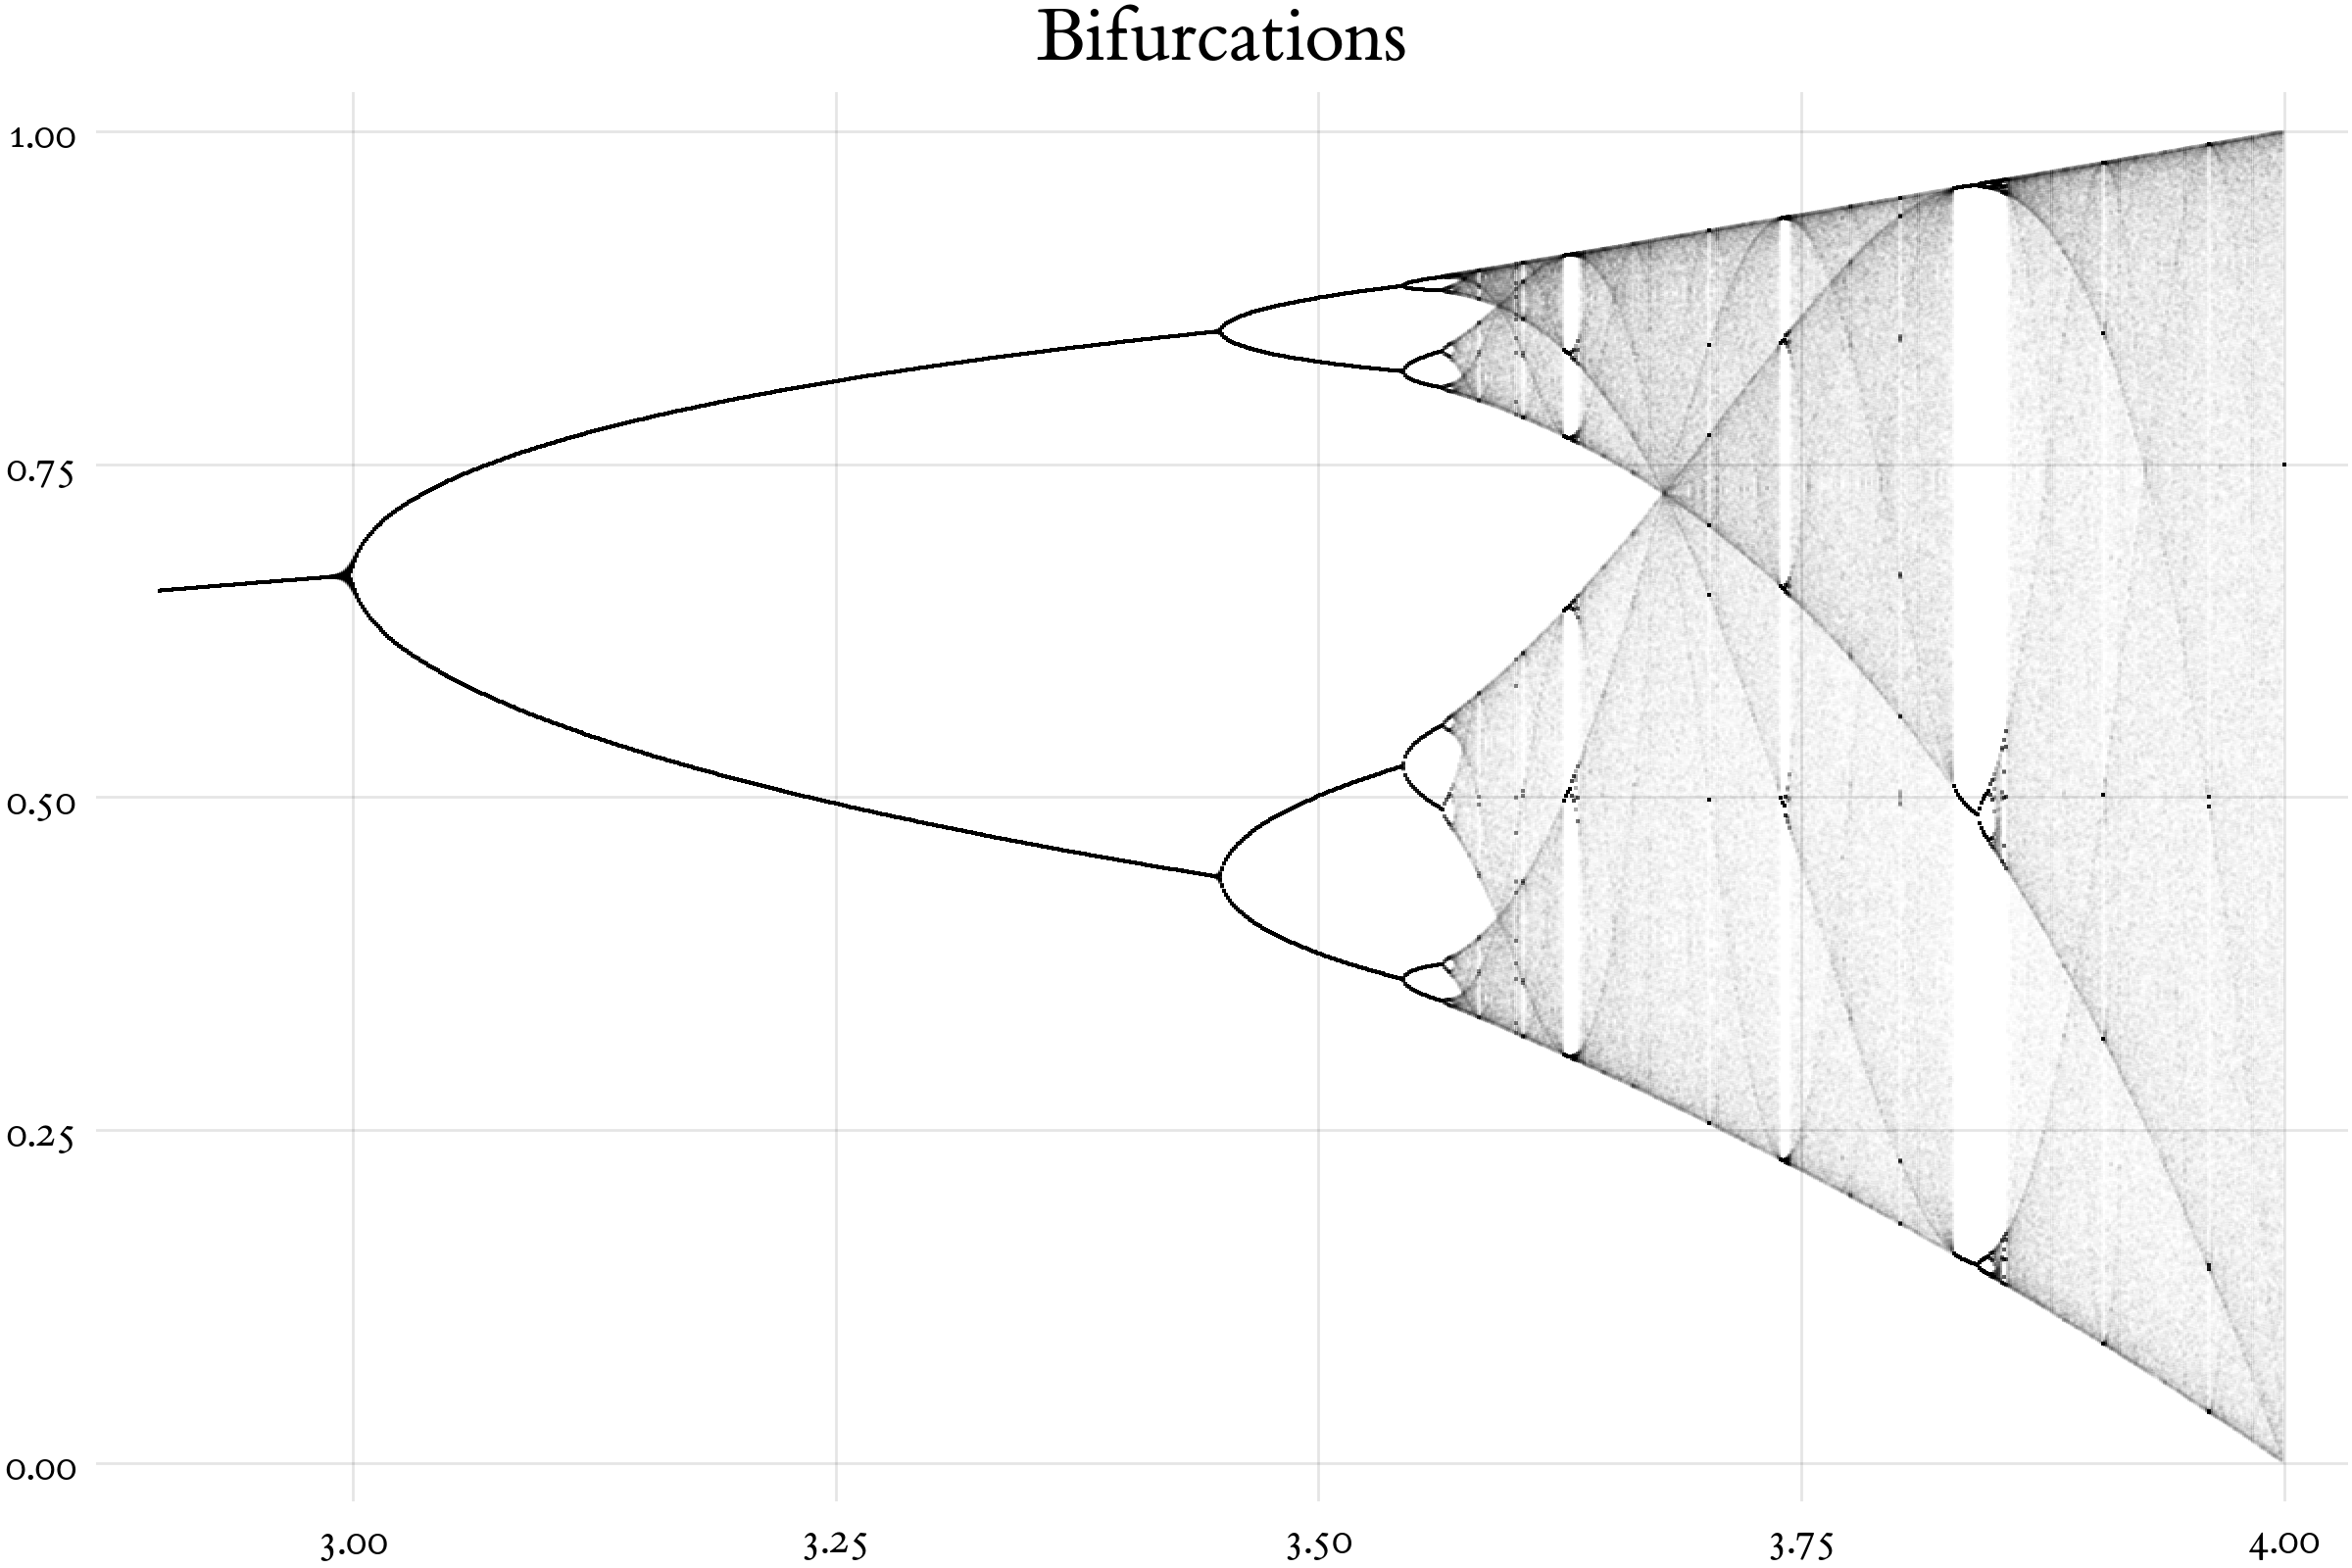
\includegraphics[width=.9\linewidth]{./bifurcation.png}
\end{figure*}

\subsection{Part 3}
\label{sec:org165a893}
\begin{minted}[frame=lines,linenos=true,mathescape,breaklines=true]{julia}
   using Base.Threads
   n = 150

   function calc_parallel(n, rs; warmup=400)
       out = zeros(n, length(rs), 2)
       to_iter = collect(enumerate(rs))

       @threads for (i, r) in to_iter
           out[:, i, 1] .= r
           slice = @view out[:, i, 2]
           calc_attractor!(slice, r, warmup=warmup)
       end
       out
   end

   println("threads: ", nthreads())
   print("serial:  ")
   @time   calc_serial(n, rs)
   print("parallel:")
   @time calc_parallel(n, rs)
   nothing
\end{minted}

\begin{verbatim}
threads: 8
serial:    0.001584 seconds (1.11 k allocations: 2.587 MiB)
parallel:  0.084049 seconds (203.27 k allocations: 12.628 MiB, 25.77% gc time)
\end{verbatim}


Currently the serial execution is much faster than the parallel execution. This is because the \texttt{@threads} macro spins up new threads
every time it is called; most of that timing overhead comes from the time it takes the OS to create and destroy threads.

If we give the threads more work to do, the ratio changes:

\begin{minted}[frame=lines,linenos=true,mathescape,breaklines=true]{julia}
   print("serial:  ")
   @time   calc_serial(n, rs, warmup=1000000)
   print("parallel:")
   @time calc_parallel(n, rs, warmup=1000000)
   nothing
\end{minted}

\begin{verbatim}
serial:    2.511244 seconds (4.80 k allocations: 2.785 MiB)
parallel:  0.550213 seconds (5.02 k allocations: 2.817 MiB)
\end{verbatim}


Now the actual computation loop dominates and the parallel implementation is much faster.

\subsection{Part 4}
\label{sec:orge4a9969}
\begin{minted}[frame=lines,linenos=true,mathescape,breaklines=true]{julia}
   using Distributed
   n = 150

   addprocs(8)

   @everywhere begin
       function calc_attractor!(out,r;warmup=400,x0=0.25)
           x = x0
           for _ in 1:warmup
               x = r * x * (1 - x)
           end
           for i in 1:length(out)
               out[i] = x
               x = r * x * (1 - x)
           end
       end
   end
   function calc_pmap(n, rs; warmup=400)
       to_iter = collect(enumerate(rs))

       function op(elem)
           i, r = elem
           slice = zeros(n)
           calc_attractor!(slice, r, warmup=warmup)
           slice
       end
       pmap(op, to_iter)
   end

   function calc_distributed(n, rs; warmup=400)
       out = zeros(n, length(rs), 2)
       to_iter = collect(enumerate(rs))

       @sync @distributed for (i, r) in to_iter
           out[:, i, 1] .= r
           slice = @view out[:, i, 2]
           calc_attractor!(slice, r, warmup=warmup)
       end
       out
   end

   print("serial:      ")
   @time   calc_serial(n, rs)
   print("pmap:        ")
   @time calc_pmap(n, rs)
   print("@distributed:")
   @time calc_distributed(n, rs)
   nothing
\end{minted}

\begin{verbatim}
serial:        0.179373 seconds (213.12 k allocations: 13.057 MiB, 69.30% gc time)
pmap:          2.105161 seconds (479.18 k allocations: 26.831 MiB, 3.39% gc time)
@distributed:  2.479598 seconds (219.67 k allocations: 14.684 MiB)
\end{verbatim}

\subsection{Part 5}
\label{sec:orgdad3180}
Serial is most efficient for small data. Parallel is best when there's a little more work; and eventually you could scale out with distributed, if you really needed to. It's a question of when the parallel speedup overpowers the constant factor.

\newpage
\section{Extra}
\label{sec:org463b922}
Some other random stuff I did trying to understand newton's method.

\begin{minted}[frame=lines,linenos=true,mathescape,breaklines=true]{julia}
  g(x) = sin.(x)

  function newton(g, x0, n=10)
      out = zeros(length(x0), n)
      x = x0
      for i in 1:n
          out[:, i] = x
          dg = ForwardDiff.jacobian(g, x)
          x = x - dg \ g(x)
      end
      return out
  end

  function quasinewton(g, x0, n=10)
      out = zeros(length(x0), n)
      x = x0
      dg = ForwardDiff.jacobian(g, x)
      for i in 1:n
          out[:, i] = x
          x = x - dg \ g(x)
      end
      return out
  end

  function newtonplot(g, x0; n=10, op=newton, title="newton's method", xstar=0)
    n = 10

    xs = op(g, [x0], n)
    ys = g.(xs)
    xs = xs[:]
    ys = ys[:]

    p = plot(sin, range(-3.0, 3.0, length=100), xlim=(-pi, pi), legend=false, title=title, foreground_color_border=:transparent, foreground_color_axis=:transparent)

    for i in 1:n-1
        plot!(p, Shape([ (xs[i], 0), (xs[i], ys[i]) ]), linecolor=:orange)
        plot!(p, Shape([ (xs[i], ys[i]), (xs[i+1], 0) ]))
    end
    plot!(p, [xs[1]], [0.], marker=true, markerstrokewidth=0)

    if abs(xstar - xs[n]) < .01
      plot!(p, [xstar], [0.], marker=true, markercolor=RGB(.3,.9,0.), markerstrokewidth=0, markersize=5.)
    else
      plot!(p, [xstar], [0.], marker=true, markercolor=:red, markerstrokewidth=0, markersize=5.)
    end
    xs = op(g, [x0], n)
    ys = g.(xs)
    xs = xs[:]
    ys = ys[:]

    p = plot(sin, range(-3.0, 3.0, length=100), xlim=(-pi, pi), legend=false, title=title, foreground_color_border=:transparent, foreground_color_axis=:transparent)

    for i in 1:n-1
        plot!(p, Shape([ (xs[i], 0), (xs[i], ys[i]) ]), linecolor=:orange)
        plot!(p, Shape([ (xs[i], ys[i]), (xs[i+1], 0) ]))
    end
    plot!(p, [xs[1]], [0.], marker=true, markerstrokewidth=0)

    if abs(xstar - xs[n]) < .01
      plot!(p, [xstar], [0.], marker=true, markercolor=RGB(.3,.9,0.), markerstrokewidth=0, markersize=5.)
    else
      plot!(p, [xstar], [0.], marker=true, markercolor=:red, markerstrokewidth=0, markersize=5.)
    end

    p
  end

  png(plot(newtonplot(g, 1.0, op=newton), newtonplot(g, 1.0, op=quasinewton, title="quasinewton method"), layout=(2,1), format=:png, dpi=200, fontfamily="ETBookOT"), "comparison.png")
\end{minted}

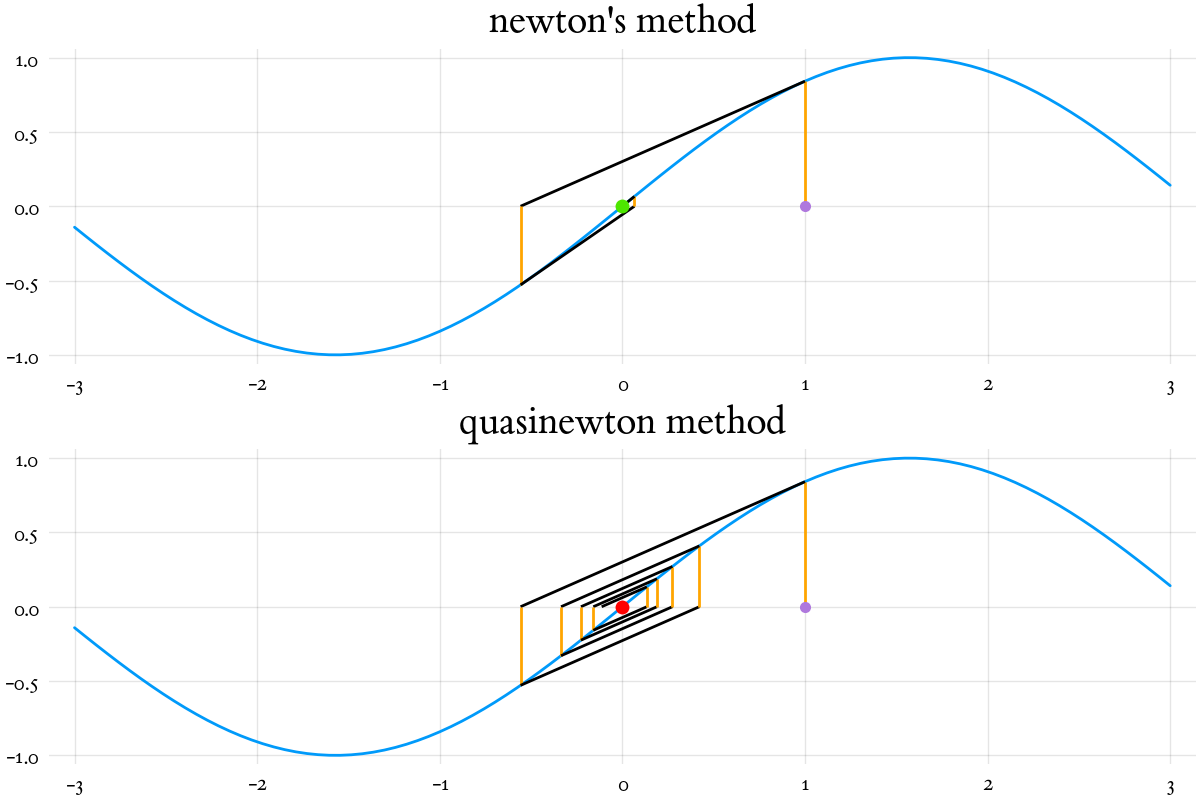
\includegraphics[width=.9\linewidth]{./comparison.png}

\begin{minted}[frame=lines,linenos=true,mathescape,breaklines=true]{julia}
  anim = @animate for y in range(0, 2pi, length=180)
    x = cos(y) * 1.3
    plot(newtonplot(g, x, op=newton), newtonplot(g, x, op=quasinewton, title="quasinewton method"), layout=(2,1), dpi=200)
  end

  gif(anim, "newton.gif")
  nothing
\end{minted}

Link to the generated gif: \url{https://i.imgur.com/vwmc64u.mp4}
\end{document}
